\documentclass{report}
% Include all project wide packages here.
\usepackage{fullpage}
\usepackage[style=ieee]{biblatex}
\usepackage[dutch]{babel}

\renewcommand{\familydefault}{\sfdefault}

\setmainfont[Ligatures=TeX]{Myriad Pro}
\setmathfont{Asana Math}
\setmonofont{Lucida Console}

\usepackage{titlesec, blindtext, color}
\definecolor{gray75}{gray}{0.75}
\newcommand{\hsp}{\hspace{20pt}}
\titleformat{\chapter}[hang]{\Huge\bfseries}{\thechapter\hsp\textcolor{gray75}{|}\hsp}{0pt}{\Huge\bfseries}
\renewcommand{\familydefault}{\sfdefault}
\renewcommand{\arraystretch}{1.2}
\setlength\parindent{0pt}

%For code listings
\definecolor{black}{rgb}{0,0,0}
\definecolor{browntags}{rgb}{0.65,0.1,0.1}
\definecolor{bluestrings}{rgb}{0,0,1}
\definecolor{graycomments}{rgb}{0.4,0.4,0.4}
\definecolor{redkeywords}{rgb}{1,0,0}
\definecolor{bluekeywords}{rgb}{0.13,0.13,0.8}
\definecolor{greencomments}{rgb}{0,0.5,0}
\definecolor{redstrings}{rgb}{0.9,0,0}
\definecolor{purpleidentifiers}{rgb}{0.01,0,0.01}


\lstdefinestyle{csharp}{
language=[Sharp]C,
showspaces=false,
showtabs=false,
breaklines=true,
showstringspaces=false,
breakatwhitespace=true,
escapeinside={(*@}{@*)},
columns=fullflexible,
commentstyle=\color{greencomments},
keywordstyle=\color{bluekeywords}\bfseries,
stringstyle=\color{redstrings},
identifierstyle=\color{purpleidentifiers},
basicstyle=\ttfamily\small}

\lstdefinestyle{c}{
language=C,
showspaces=false,
showtabs=false,
breaklines=true,
showstringspaces=false,
breakatwhitespace=true,
escapeinside={(*@}{@*)},
columns=fullflexible,
commentstyle=\color{greencomments},
keywordstyle=\color{bluekeywords}\bfseries,
stringstyle=\color{bluestrings},
identifierstyle=\color{purpleidentifiers}
}

\lstdefinestyle{vhdl}{
language=VHDL,
showspaces=false,
showtabs=false,
breaklines=true,
showstringspaces=false,
breakatwhitespace=true,
escapeinside={(*@}{@*)},
columns=fullflexible,
commentstyle=\color{greencomments},
keywordstyle=\color{bluekeywords}\bfseries,
stringstyle=\color{redstrings},
identifierstyle=\color{purpleidentifiers}
}

\lstdefinestyle{xaml}{
language=XML,
showspaces=false,
showtabs=false,
breaklines=true,
showstringspaces=false,
breakatwhitespace=true,
escapeinside={(*@}{@*)},
columns=fullflexible,
commentstyle=\color{greencomments},
keywordstyle=\color{redkeywords},
stringstyle=\color{bluestrings},
tagstyle=\color{browntags},
morestring=[b]",
  morecomment=[s]{<?}{?>},
  morekeywords={xmlns,version,typex:AsyncRecords,x:Arguments,x:Boolean,x:Byte,x:Char,x:Class,x:ClassAttributes,x:ClassModifier,x:Code,x:ConnectionId,x:Decimal,x:Double,x:FactoryMethod,x:FieldModifier,x:Int16,x:Int32,x:Int64,x:Key,x:Members,x:Name,x:Object,x:Property,x:Shared,x:Single,x:String,x:Subclass,x:SynchronousMode,x:TimeSpan,x:TypeArguments,x:Uid,x:Uri,x:XData,Grid.Column,Grid.ColumnSpan,Click,ClipToBounds,Content,DropDownOpened,FontSize,Foreground,Header,Height,HorizontalAlignment,HorizontalContentAlignment,IsCancel,IsDefault,IsEnabled,IsSelected,Margin,MinHeight,MinWidth,Padding,SnapsToDevicePixels,Target,TextWrapping,Title,VerticalAlignment,VerticalContentAlignment,Width,WindowStartupLocation,Binding,Mode,OneWay,xmlns:x}
}

%defaults
\lstset{
basicstyle=\ttfamily\small,
extendedchars=false,
numbers=left,
numberstyle=\ttfamily\tiny,
stepnumber=1,
tabsize=4,
numbersep=5pt
}
\addbibresource{../../library/bibliography.bib}

\title{EPO-2: Mid-term Design Report - Aansturing Servomotoren}
\author{Robin Hes}

\begin{document}

\chapter{Aansturing Servomotoren}
\label{ch:servo}

De belangrijkste actuators in het ontwerp zijn de servomotoren die de wielen van de robot aandrijven.
Zonder deze servo's zou de robot vanzelfsprekend niet van zijn plek af komen.
Beide motoren worden onafhankelijk aangestuurd en verzorgen niet alleen de voortstuwing, maar ook de besturing van de robot.
De servo's worden aangestuurd door de FPGA op de robot, middels een pulse-width modulation-signaal (PWM-signaal).
Dit signaal moet in de FPGA gegenereerd worden en aan de volgende eisen voldoen:

\section{Eisen}
\label{sec:servo-eisen}

\begin{itemize}
	\item De frequentie van het signaal moet gelijk zijn aan 50 Hz
	\item De duty-cycle moet tussen de 5 en 10 \% (1.0 en 2.0 ms) liggen
	\item Het pulssignaal moet tussen de 3 en 5 V liggen
\end{itemize}

\noindent
Verder geldt het volgende voor wat betreft de draairichting van de servo's:

\begin{itemize}
	\item Van bovenaf gezien draait de servo bij pulswijdtes onder de 1.5 ms met de klok mee
	\item Van bovenaf gezien draait de servo bij pulswijdtes boven de 1.5 ms tegen de klok in
	\item Bij een pulswijdte van exact 1.5 ms staat de servo stil
\end{itemize}

\section{Ontwerp en implementatie}
\label{sec:servo-design}

Er moet dus een pulsgenerator gebouwd worden die afhankelijk van de gewenste snelheid per wiel een geschikte pulswijdte maakt.
Een pulsgenerator als deze is vrij gemakkelijk te realiseren in een FPGA, door simpelweg het uitgangssignaal van de motorcontrol een bepaalde tijd op '1' te zetten (de puls) en daarna gedurende de rest van de periode van het PWM-signaal weer op '0'.
De eerste stap is dan het bepalen van de pulswijdte.
Als uitganspunt kan hiervoor de pulswijdte gebruikt worden waarop de servo stil staat: 1.5 ms.
Deze tijdsduur staat gelijk aan $1.5 \cdot 10^{-3} \cdot 50 \cdot 10^{6} = 75000$ klokpulsen.
Voor voor- en achteruit wijkt de pulswijdte hier maximaal $\pm$ 0.5 ms van af, oftewel $0.5 \cdot 10^{-3} \cdot 50 \cdot 10^{6} = 25000$ klokpulsen.
Voor het generen van een eenvoudig PWM-signaal met standen ``vooruit'', ``achteruit'' en ``stilstaan'' hoeven er dus alleen maar klokpulsen geteld te worden, waarna het uitgangssignaal (afhankelijk van de positie van de sensor) bij respectievelijk $75000 + 25000 = 100000$, $75000 - 25000 = 50000$ en $75000 + 0 = 75000$ klokpulsen op '0' gezet wordt, hiervoor was het signaal dan vanzelfsprekend '1'.
Omdat het wenselijk is dat er ook snelheden tussen vol vooruit en vol achteruit aangehouden moeten kunnen worden werken wij met een basispulswijdte van 75000 klokpulsen, waar dan vervolgens een factor van 0-100 maal 250 bij opgeteld of van afgetrokken wordt.
De formule voor het aantal klokpulsen waarvoor het signaal '1' is wordt dan:

\begin{equation}
	\label{eq:pulsewidth}
	N = 75000 + 250 \cdot speed;\quad -100 \leq speed \leq 100
\end{equation}

Een totaal overzicht van de aansturing van de servo kan schematisch als volgt worden weergegeven:

\begin{figure}[H]
	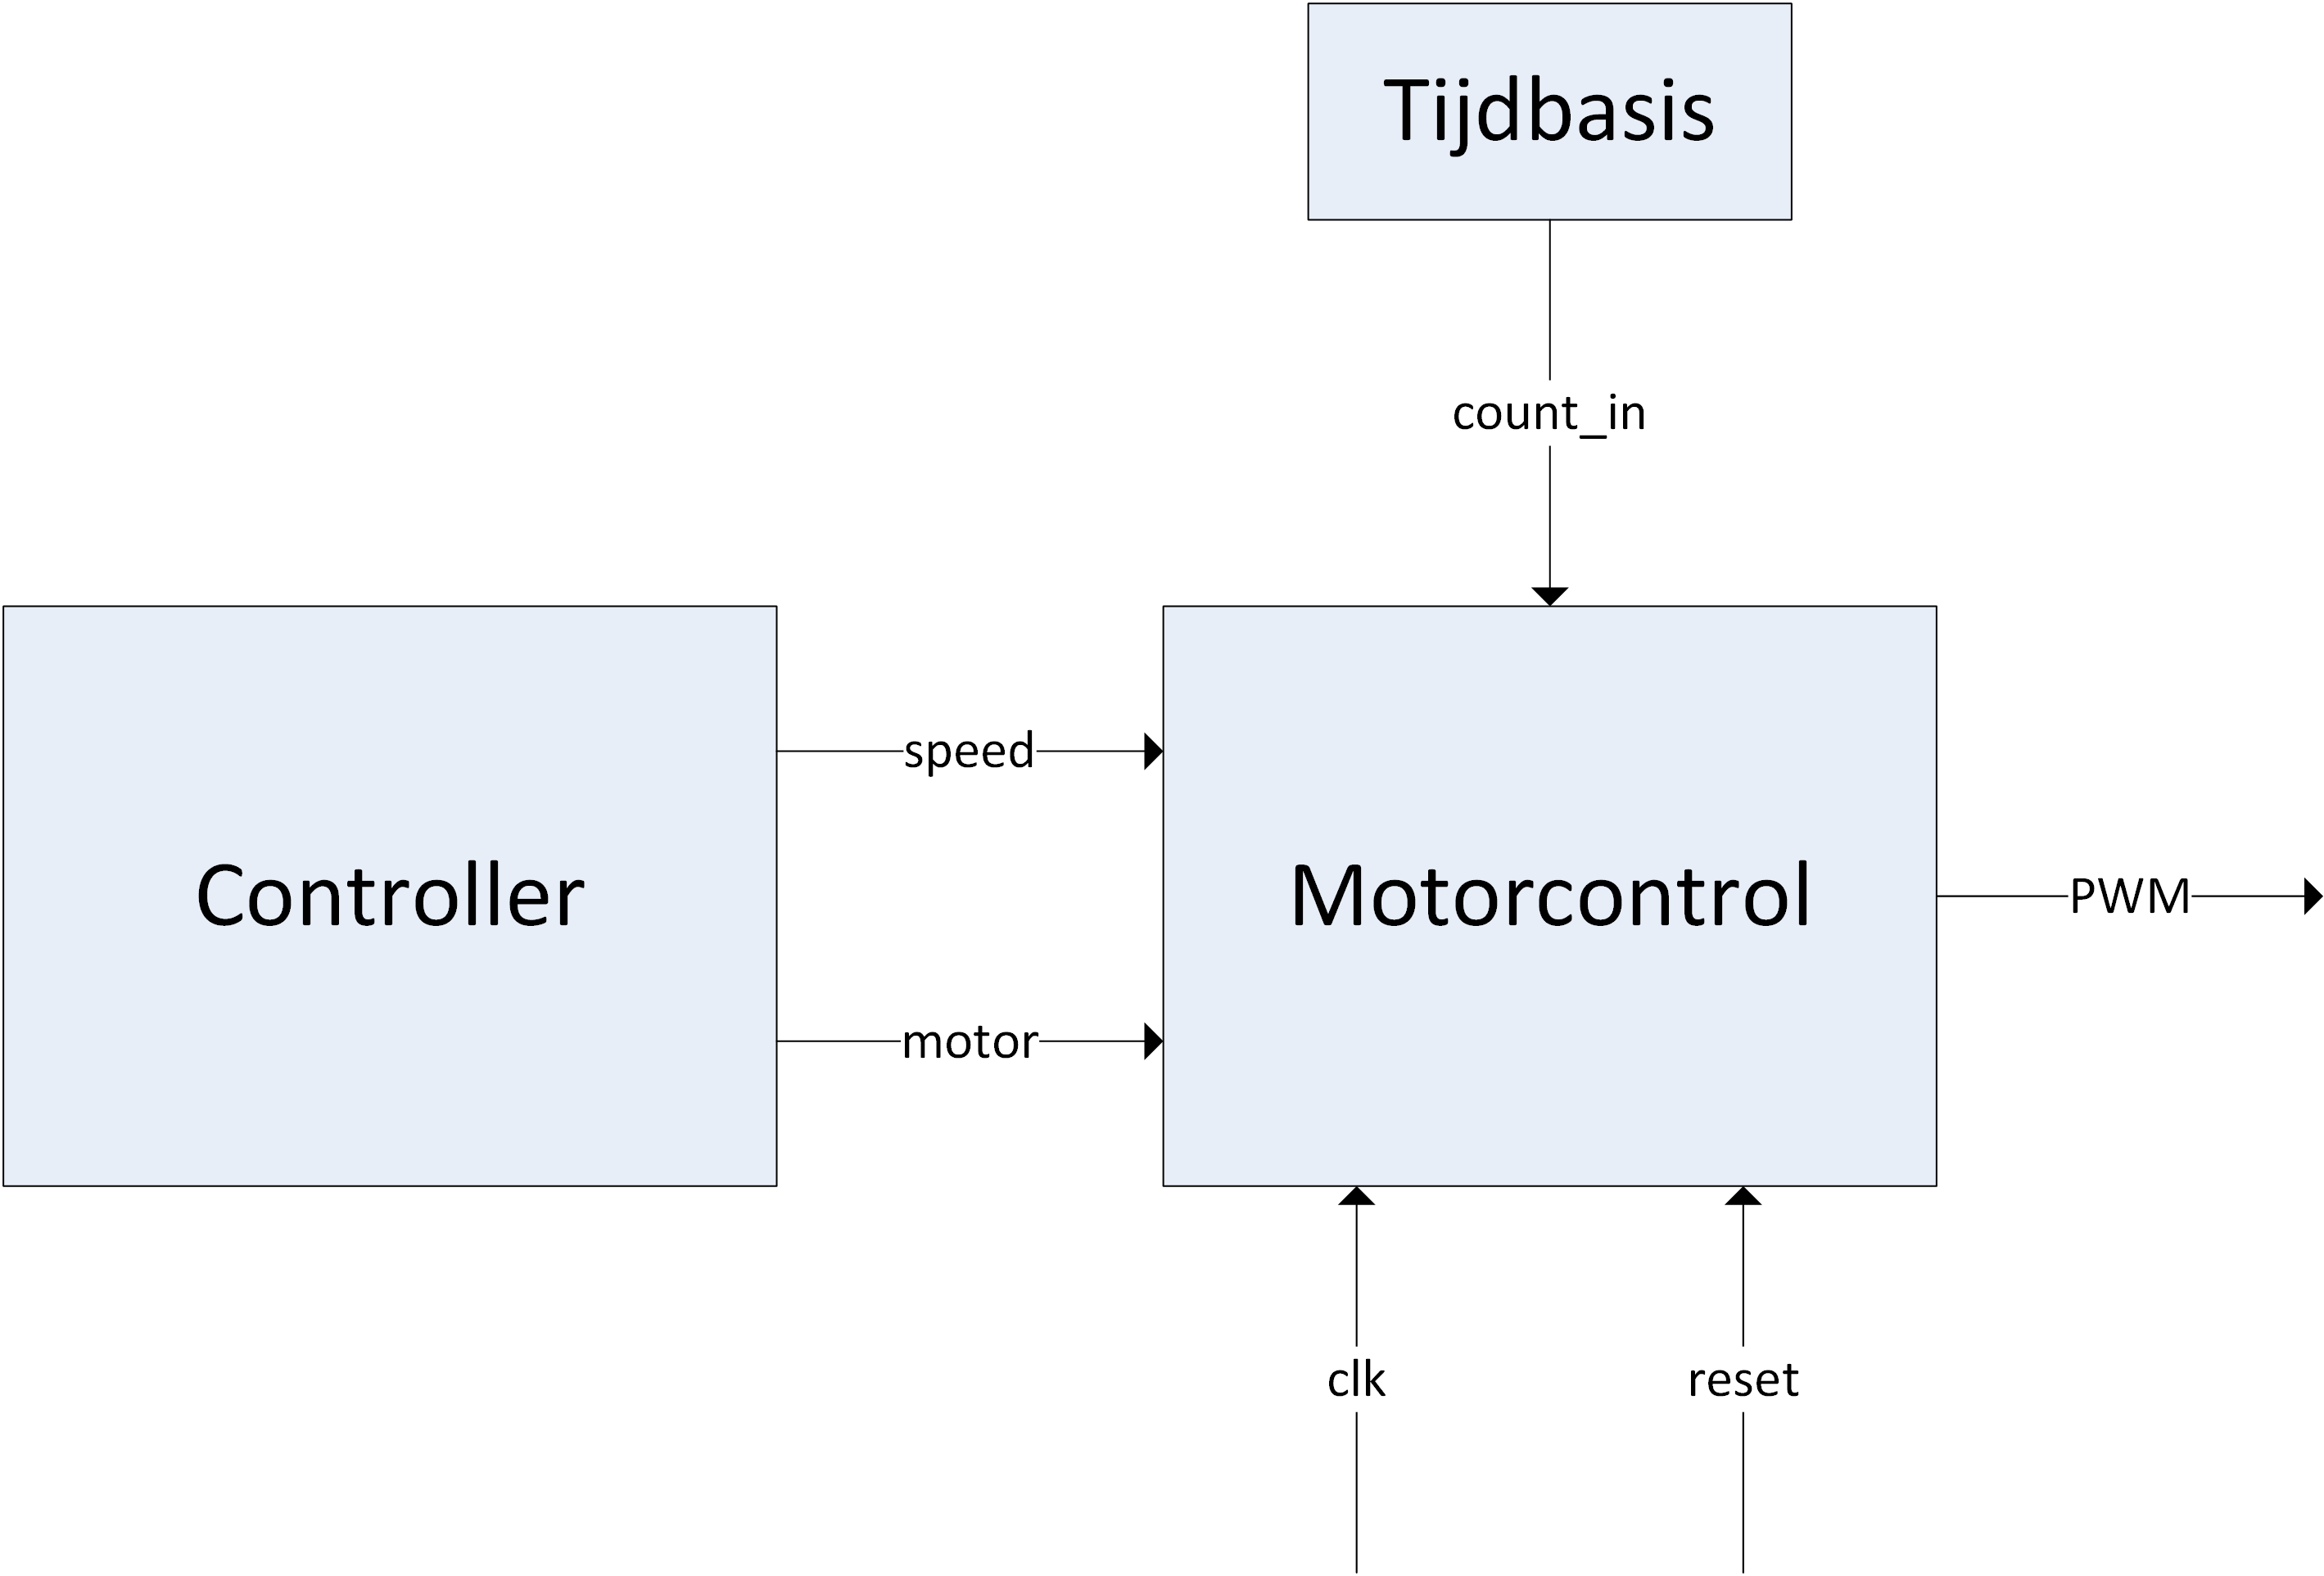
\includegraphics[width=\textwidth]{resource/motor-control}
	\caption{Schematisch overzicht van de motoraansturing}
	\label{fig:motorcontrol}
\end{figure}

De structurele opbouw van het motorsysteem is grotendeels overgenomen uit de gegeven vhdl-bestanden en ziet er als volgt uit:
De architectuur voor de pulsenteller die het aantal verstreken klokpulsen bijhoudt, bevindt zich in \textit{timebase.vhdl} (zie bijlage \ref{appsec:timebase.vhdl}), de controller die de gewenste pulswijdte vergelijkt met het aantal verstreken klokpulsen in \textit{motorcontrol.vhdl} (zie bijlage \ref{appsec:motorcontrol.vhdl}).
Het klok- en resetsignaal (\textit{clk} en \textit{reset}) zijn inputs van buitenaf, de gewenste snelheid (\textit{speed}) en de motor (links of rechts) voor welke het signaal moet worden gegenereerd worden (\textit{motor}) aangeleverd door de overkoepelende controller (\textit{controller.vhdl}, zie bijlage \ref{appsec:controller.vhdl}) en het opgetelde aantal klokpulsen wordt door timebase aan motorcontrol geleverd middels het signaal \textit{count\_in}.

\section{Test}
\label{sec:servo-test}

Om de motoraansturing te toetsen aan de vereisten, hebben we eerst een testbench geschreven om mee te simuleren in modelsim. Deze testbench is te vinden in bijlage \ref{appsec:motorcontrol-tb.vhdl} 

\begin{figure}[H]
	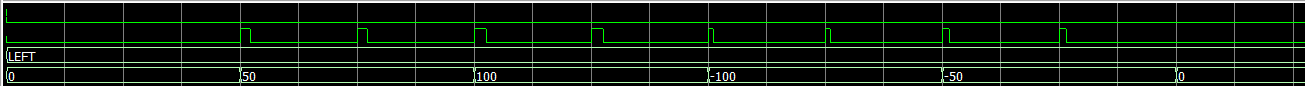
\includegraphics[width=\textwidth]{resource/motor-control-sim}
	\caption{Simulatie van de motoraansturing in Modelsim voor verschillende snelheden. Iedere kolom staat voor $10 \mathrm{ms}$, de rijen stellen van boven naar beneden de signalen \textit{reset}, \textit{pwm}, \textit{motor}, \textit{speed} voor.}
	\label{fig:motorcontrol-sim}
\end{figure}

In figuur \ref{fig:motorcontrol-sim} is te zien dat de pulswijdte in de simulatie correct aangepast wordt wanneer de snelheid aangepast wordt. Ook is de periode gelijk aan $20 \mathrm{ms}$. Tot slot zien we dat bij de maximale snelheid van 100, de pulswijdte gelijk is aan $2.0 \mathrm{ms}$ en bij de minimale snelheid van -100, de pulswijdte gelijk is aan $1.0 \mathrm{ms}$. Hiermee worden de duty-cycle limieten niet overschreden en is dus aan alle eisen voldaan.

\begin{figure}[H]
	\centering
	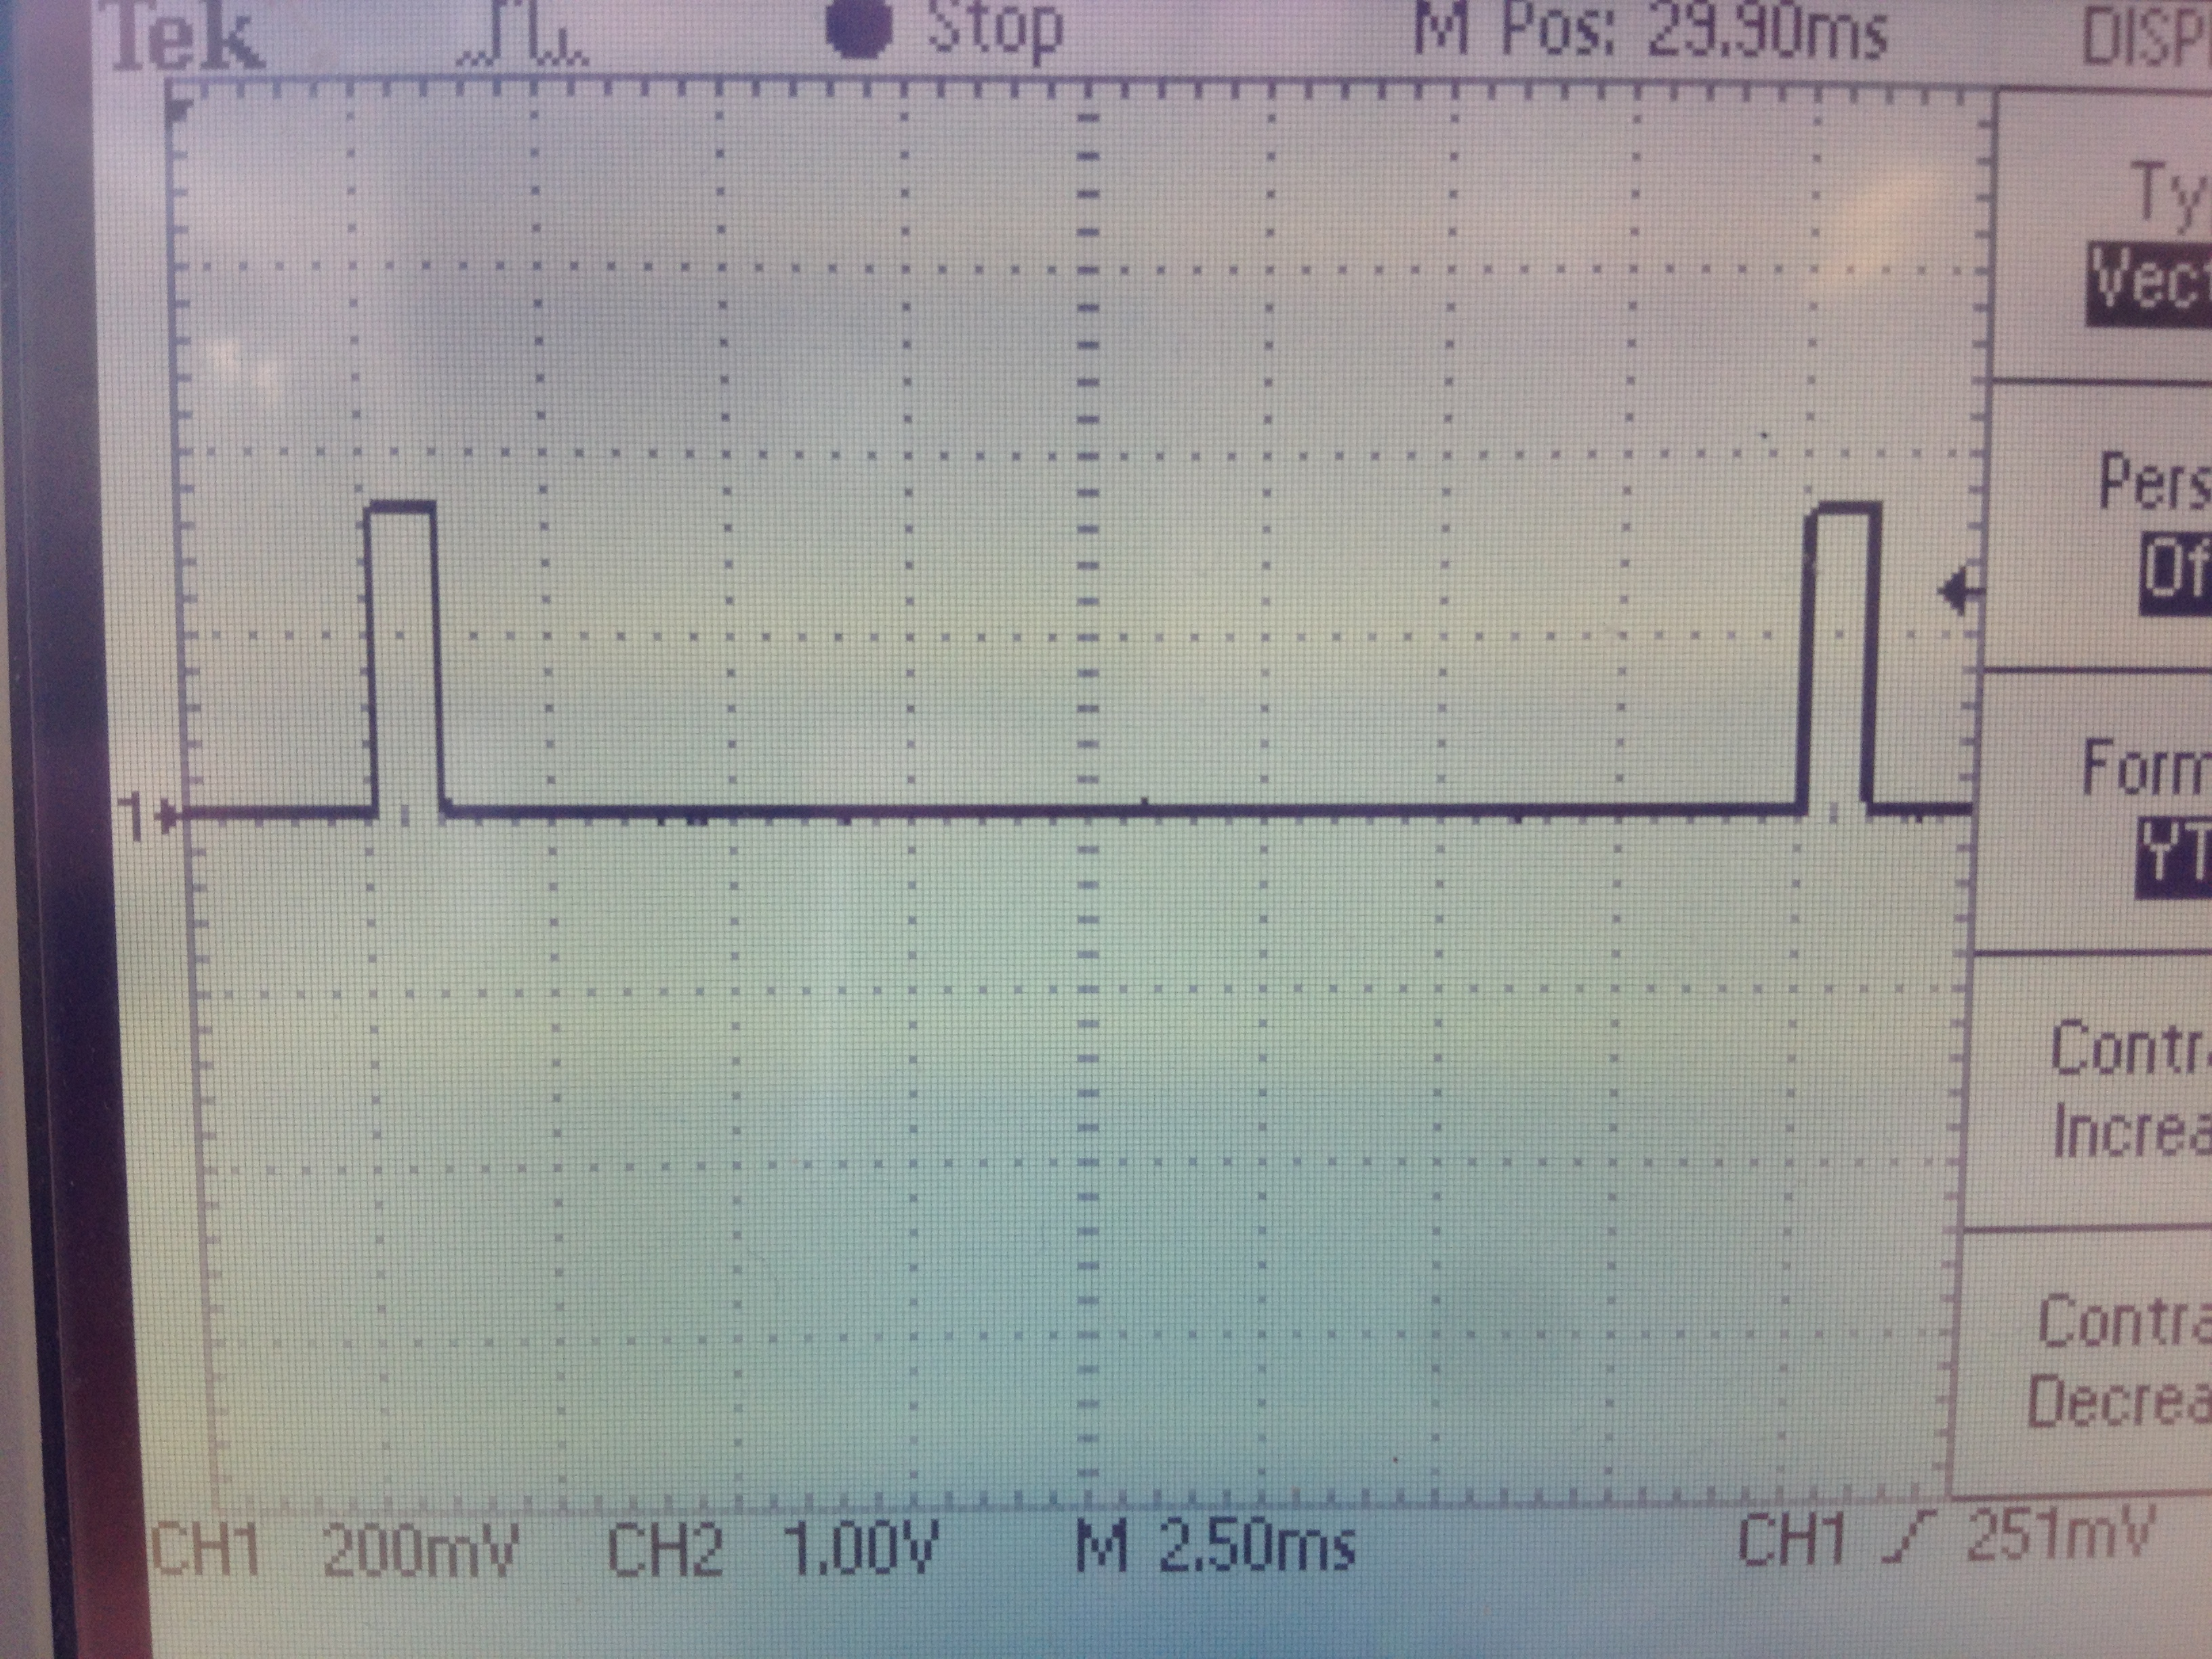
\includegraphics[width=0.5\textwidth]{resource/motor-control-scoop}
	\caption{Test van de motoraansturing op de FPGA, bij een snelheid van 100}
	\label{fig:motorcontrol-scoop}
\end{figure}

Vervolgens hebben we de VHDL op de FPGA geladen en een oscilloscoop aan de pin-out voor één van de servo's gehangen en de verschillende snelheden getest. Het resultaat van de test bij een snelheid van 100 (een periode van $2.0\mathrm{ms}$) is te vinden in figuur \ref{fig:motorcontrol-scoop}. Ook hier zijn de resultaten conform de eisen.

\section{Discussie}
\label{sec:servo-disc}

Het signaal wordt correct gegenereerd, met de juiste periode, pulswijdten en spanningsniveau's.
Daarnaast kunnen we de robot aansturen op een door ons gekozen snelheid.
Het ontwerp en onze implementatie van de servoaansturing is dus functioneel en voldoet aan alle gestelde eisen.

\end{document}